\section{Theorie}
\label{sec:Theorie}

\subsection{Lichtbrechung an einer Grenzfläche}
Wenn Licht auf eine Grenzfläche von zwei Medien trifft, wird es teilweise
reflektiert und teilweise transmittiert. Das Ausmaß von Reflexion und
Transmission hängt vom Einfallswinkel und den Brechungsindizes der beteiligten
Materialien ab. Nach dem Reflexionsgesetz ist der Einfallswinkel gleich dem
Reflexionswinkel ($\alpha_1 = \alpha_2$), während die Richtung des transmittierten
Lichts durch das Snellius'sche Brechungsgesetz bestimmt wird: 
\begin{equation}
    \label{eqn:1}
    n_1 \, \sin(\alpha_1) = n_2 \, \sin(\alpha_2)
\end{equation}
\noindent Die Intensitätsverteilung zwischen 
reflektiertem und transmittiertem Licht wird durch die Fresnel-Gleichungen
beschrieben, die auch die Polarisation des Lichts berücksichtigen. Diese 
sollen in \autoref{subsec:senk} und \autoref{subsec:para} weiter thematisiert 
sein. In \autoref{fig:1} ist zu sehen, wie die Brechung des Lichts aussieht.
\begin{figure}[H]
    \caption{Transmission und Reflexion an einer Grenzfläche.\cite{anleitung8}}
    \centering
    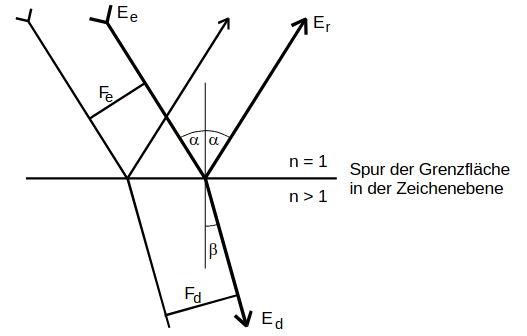
\includegraphics[width=0.7\textwidth]{"Bilder/brechung.png"}
    \label{fig:1}
\end{figure}
\noindent Der Feldvektor für die einlaufende Welle ist gegeben durch einen 
senkrechten und einen parallelen Teil:
\begin{equation}
    \label{eqn:2}
    \vec{E_e} = \vec{E_{\perp}} + \vec{E_{\parallel}}.
\end{equation}
Aus der Elektrodynamik ist bekannt, dass die tangentiale Komponente des elektrishen 
Feldes an der Grenzfläche stetig ist. Damit ergibt sich, dass die senkrechten 
Komponenten der einfallenden und reflektierten Welle gleich dem senkrechten 
Anteil der transmittierten Welle sein müssen.
\begin{equation}
    \label{eqn:3}
    \vec{E_{d_\perp}} = \vec{E_{e_\perp}} + \vec{E_{r_\perp}}
\end{equation}
Ebenso gilt diese Gleichung für parallele Polarisation:
\begin{equation}
    \label{eqn:4}
    \vec{E_{d_\parallel}} = \vec{E_{e_\parallel}} + \vec{E_{r_\parallel}}.
\end{equation}
Im Folgenden wird angenommen, dass die Materialien nicht-ferromagnetisch
sind, was zur Folge hat, dass die magnetische Permeabilität $\mu \approx 1$ und 
die Stromdichte $\vec{j}=0$ ist. Darüber hinaus ist der Betrag des Poynting-
Vektors, welcher die Strahlungsleistung pro Flächeineinheit eines Feldes beschreibt, 
gegeben durch:
\begin{equation}
    \label{eqn:5}
    |\vec{S}| = |v \varepsilon \varepsilon_0 \vec{E}^2|
\end{equation}

\subsection{Senkrechte Polarisation}
\label{subsec:senk}
Bei senkrechter Polarisation schwingt das elektrische Feld senkrecht zur 
Einfallsebene und parallel zur Grenzfläche.
Aus der Stetigkeitsbedingung aus \autoref{eqn:3} und dem Snelliusschen Brechungsgesetz 
mit $n1=n2$ ergibt sich die Relation 
\begin{equation}
    \label{eqn:6}
    \vec{E_{r_\perp}}(\alpha) = \vec{E_{e_\perp}} \frac{(\sqrt{n^2-\sin(\alpha)^2} - 
    \cos(\alpha))^2}{n^2 - 1}
\end{equation}
für die Intensität des reflektierten Lichtstrahls.

\subsection{Parallele Polarisation}
\label{subsec:para}
Diese Art der Polarisation liegt vor, wenn das elektrische Feld parallel zur 
Einfallsebene schwingt und der Feldvektor dementsprechend senkrecht zur Grenzfläche 
steht. Wieder folgt aus der Stetigkeitsbedingung (\autoref{eqn:4}) zusammen mit 
dem Snelliusschen Zusammenhang für gleiche Brechungsindizes
\begin{equation}
    \vec{E_{r_\parallel}}(\alpha) = \vec{E_{e_\parallel}} 
    \left|\frac{n^2 \cos(\alpha) - \sqrt{n^2-\sin(\alpha)^2}}
    {n^2 \cos(\alpha) + \sqrt{n^2-\sin(\alpha)^2}}  \right|
\end{equation}
als Gleichung für die Intensität des reflektierten Lichtes.

\subsection{Brewster-Winkel}
\label{subsec:brewster}
Der Brewster-Winkel tritt auf, wenn ein vollends senkrecht polarisierter Strahl 
auf ein Medium trifft und ein 90°-Winkel zwischen dem reflektierten und
gebrochenen Lichtstrahl liegt. Er ist definiert durch
\begin{equation}
    \label{eqn:8}
    \tan{\theta_B} = \frac{n_2}{n_1}
\end{equation}
oder als
\begin{equation}
    \label{eqn:8}
    \tan{\theta_B} = n
\end{equation}
bei den vorher angesprochenen Annahmen. Dieser Zusammenhang leitet 
sich aus der Überlegung $\theta_e + \theta_{Brechung} = 90°$ ab.